\chapter{Memento模式}
\section{Memento模式的概念}
\subsection{定义}
备忘录(Memento)模式的定义:在不破坏封装性的前提下,捕获一个对象的内部状态,并在该对象之外保存这个状态,以便以后当需要时能将该对象恢复到原先保存的状态。该模式又叫快照模式。
\subsection{优点}
\begin{enumerate}
	\item 提供了一种可以恢复状态的机制。当用户需要时能够比较方便地将数据恢复到某个历史的状态。
	\item 实现了内部状态的封装。除了创建它的发起人之外,其他对象都不能够访问这些状态信息。
	\item 简化了发起人类。发起人不需要管理和保存其内部状态的各个备份,所有状态信息都保存在备忘录中,并由管理者进行管理,这符合单一职责原则。
\end{enumerate}
\subsection{缺点}
资源消耗大。如果要保存的内部状态信息过多或者特别频繁,将会占用比较大的内存资源。
\subsection{备忘录模式的角色}
\begin{enumerate}
	\item Originator生成者(发起者):记录当前时刻的内部状态信息,提供创建备忘录和恢复备忘录数据的功能,实现其他业务功能,它可以访问备忘录里的所有信息。
	\item Memento备忘录:负责存储发起人的内部状态,在需要的时候提供这些内部状态给发起人。
	两种接口:
	\begin{itemize}
		\item wide interface——宽接口:指用于获取恢复对象状态信息的方法的集合,
		只有发起者能够使用。
		\item narrow interface——窄接口,为Caretaker提供。
	\end{itemize}
	\item Caretaker管理者:对备忘录进行管理,提供保存与获取备忘录的功能,但其不能对备忘录的内容进行访问与修改。
\end{enumerate}
\subsection{应用场景}
\begin{enumerate}
	\item 需要保存与恢复数据的场景,如玩游戏时的中间结果的存档功能;
	\item 需要提供一个可回滚操作的场景,如 Word、记事本、Photoshop,Eclipse 等软件在编辑时按 Ctrl+Z 组合键,还有数据库中事务操作。
\end{enumerate}
\section{备忘录模式实现——例一}
\begin{table}[!h]
	\begin{tabular}{|l|l|l|}
		\hline
		包&名字&说明\\
		\hline
		game&Memento&Gamer状态的类\\
		\hline
		game&Gamer&游戏主人公,会生成Memento实例\\
		\hline
		&Main&测试类,会保存Memento实例,之后可以恢复\\
		\hline
	\end{tabular}
\end{table}
\begin{figure}[!h]
	\centering
	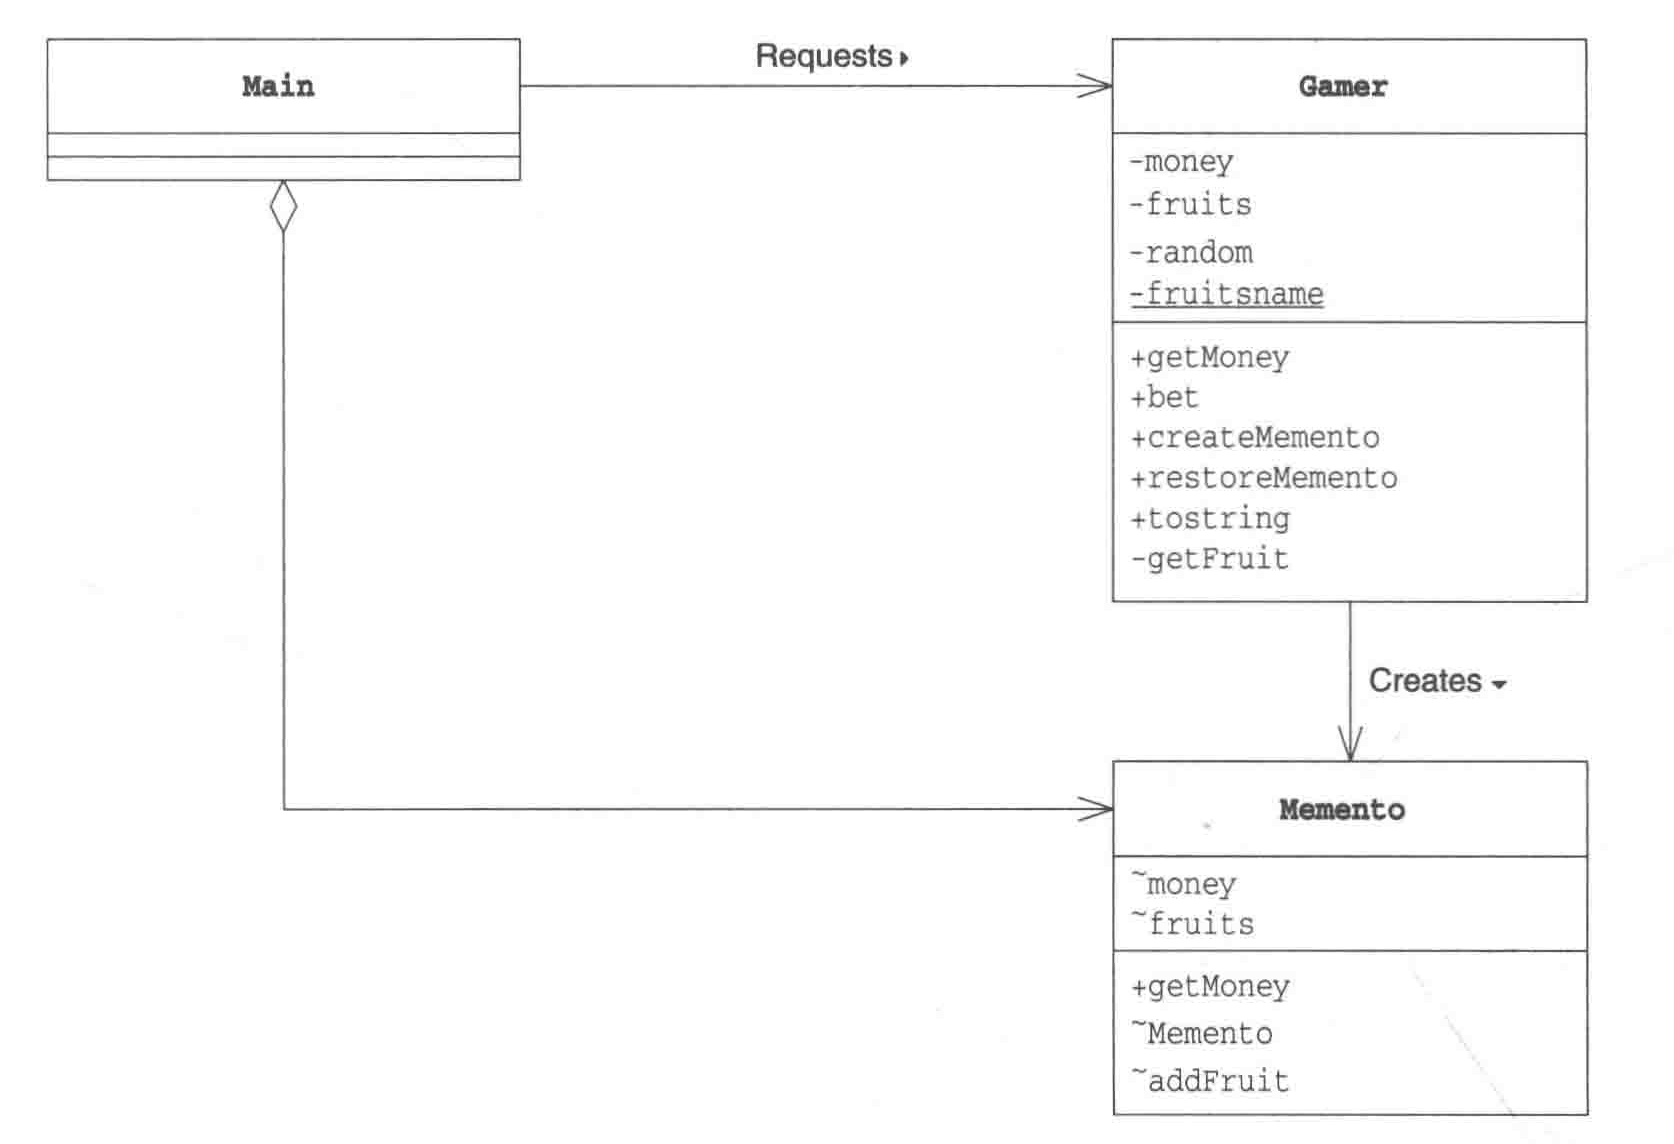
\includegraphics[width=0.8\textwidth]{image/18-1}
	\caption{备忘录模式类图}
\end{figure}
\begin{figure}[!h]
	\centering
	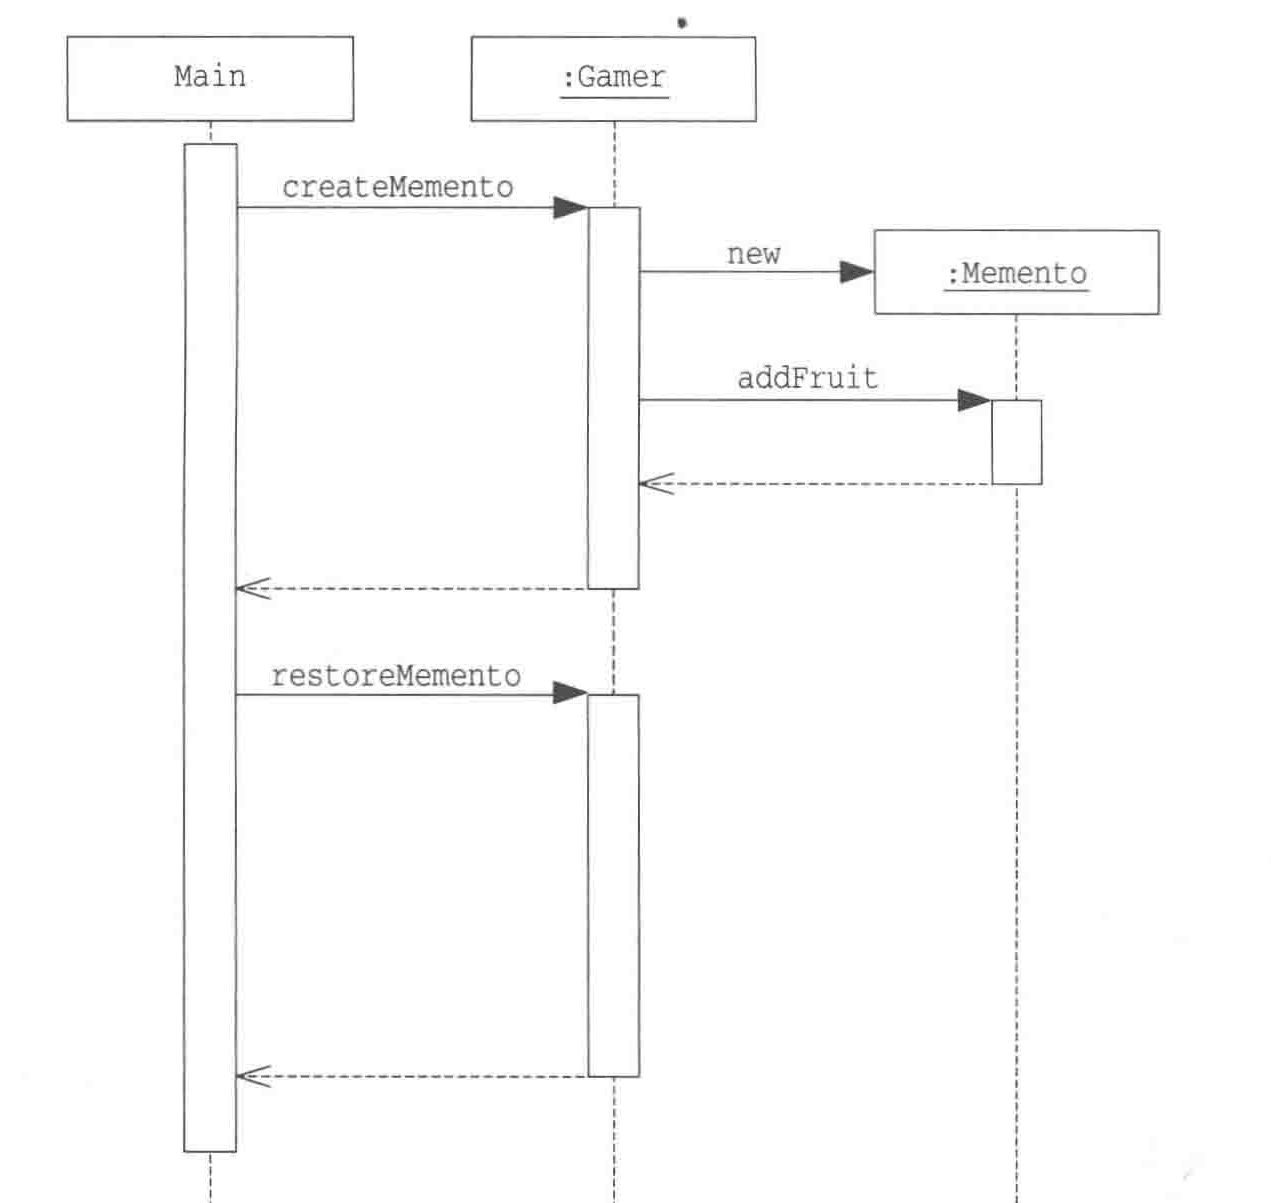
\includegraphics[width=0.6\textwidth]{image/18-2}
	\caption{备忘录模式顺序图}
\end{figure}
\begin{lstlisting}
public class Memento {
	int money;
	ArrayList<String> fruits;
	Memento(int money) {
		this.money = money;
		fruits = new ArrayList<>();
	}
	void addFruits(String fruit) {
		fruits.add(fruit);
	}
	public int getMoney() {
		return money;
	}
	List<String> getFruits() {
		return (List<String>) fruits.clone();
	}
}
\end{lstlisting}
\begin{lstlisting}
// 表示游戏主人公
public class Gamer {
	private static String[] fruitsName = {"苹果", "葡萄", "香蕉", "橘子",};
	private int money; //所持金钱
	private List<String> fruits = new ArrayList<>();    //所获得的水果
	private Random random = new Random();   //随机数生成器
	public Gamer(int money) {
		this.money = money;
	}
	public int getMoney() {
		return money;
	}
	// 掷筛子进行游戏
	public void bet() {
		int dice = random.nextInt(6) + 1;
		if (dice == 1) { //结果为一,增加金钱
			money += 100;
			System.out.println("金钱增加了");
		} else if (dice == 2) {
			money /= 2;
			System.out.println("金钱减半");
		} else if (dice == 6) {
			String f = getFruit();
			System.out.println("获得水果(" + f + ")");
		} else {
			System.out.println("什么都没有发生");
		}
	}
	// 拍摄快照
	public Memento createMemento() {
		Memento m = new Memento(money);
		Iterator<String> it = fruits.iterator();
		while (it.hasNext()) {
			String f = it.next();
			if (f.startsWith("好吃的")) {
				m.addFruits(f);
			}
		}
		return m;
	}
	// 撤销
	public void restoreMemento(Memento memento) {
		this.money = memento.money;
		this.fruits = memento.fruits;
	}
	public String toString() {
		return "Gamer{" +
			"money=" + money +
			", fruits=" + fruits +
			", random=" + random +
			'}';
	}
	private String getFruit() {
		String prefix = "";
		if (random.nextBoolean()) {
			prefix = "好吃的";
		}
		return prefix + fruitsName[random.nextInt(fruitsName.length)];
	}
}
\end{lstlisting}
\begin{lstlisting}
public class Main {
	public static void main(String[] args) {
		Gamer gamer = new Gamer(100);
		Memento memento = gamer.createMemento();
		for (int i = 0; i < 100; i++) {
			System.out.println("==== " + i);    //掷筛子的次数
			System.out.println(" 当前状态:" + gamer);
			gamer.bet();    //进行游戏
			System.out.println("所持金钱为:" + gamer.getMoney() + " 元。");
			if (gamer.getMoney() > memento.getMoney()) {
				System.out.println("(所持金额增加了,因此保存当前的状态。)");
				memento = gamer.createMemento();
			} else if (gamer.getMoney() < memento.getMoney() / 2) {
				System.out.println("所持金钱减少了,回复至之前的状态");
				gamer.restoreMemento(memento);
			}
			try {
				Thread.sleep(1000);
			} catch (InterruptedException e) {}
			System.out.println();
		}
	}
}
\end{lstlisting}
\section{备忘录模式实现——例二}
\begin{figure}[!h]
	\centering
	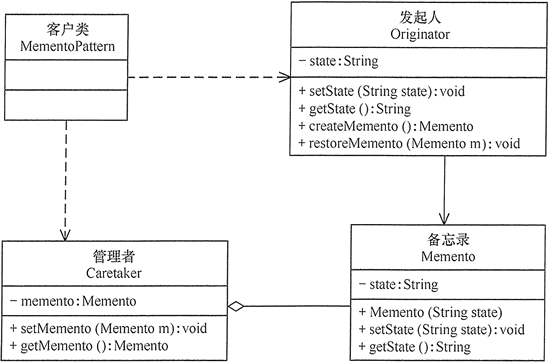
\includegraphics[width=0.6\textwidth]{image/18-3}
	\caption{备忘录模式的结构图}
\end{figure}
\begin{lstlisting}
//备忘录
class Memento {
	private String state;
	public Memento(String state) {
		this.state = state;
	}
	public void setState(String state) {
		this.state = state;
	}
	public String getState() {
		return state;
	}
}
\end{lstlisting}
\begin{lstlisting}
//发起人
class Originator {
	private String state;
	public void setState(String state) {
		this.state = state;
	}
	public String getState() {
		return state;
	}
	public Memento createMemento() {
		return new Memento(state);
	}
	public void restoreMemento(Memento m) {
		this.setState(m.getState());
	}
}
\end{lstlisting}
\begin{lstlisting}
//管理者
class Caretaker {
	private Memento memento;
	public void setMemento(Memento m) {
		memento = m;
	}
	public Memento getMemento() {
		return memento;
	}
}
\end{lstlisting}
\begin{lstlisting}
public class MementoPattern {
	public static void main(String[] args) {
		Originator or = new Originator();
		Caretaker cr = new Caretaker();
		or.setState("S0");
		System.out.println("初始状态:" + or.getState());
		cr.setMemento(or.createMemento()); //保存状态
		or.setState("S1");
		System.out.println("新的状态:" + or.getState());
		or.restoreMemento(cr.getMemento()); //恢复状态
		System.out.println("恢复状态:" + or.getState());
	}
}
\end{lstlisting}
\begin{lstlisting}
//output
初始状态:S0
新的状态:S1
恢复状态:S0
\end{lstlisting}

\section{模式扩展}
备忘录模式如何同原型模式混合使用。在备忘录模式中,通过定义“备忘录”来备份“发起人”的信息,而原型模式的 clone() 方法具有自备份功能,所以,如果让发起人实现 Cloneable 接口就有备份自己的功能,这时可以删除备忘录类。
\begin{figure}[!h]
	\centering
	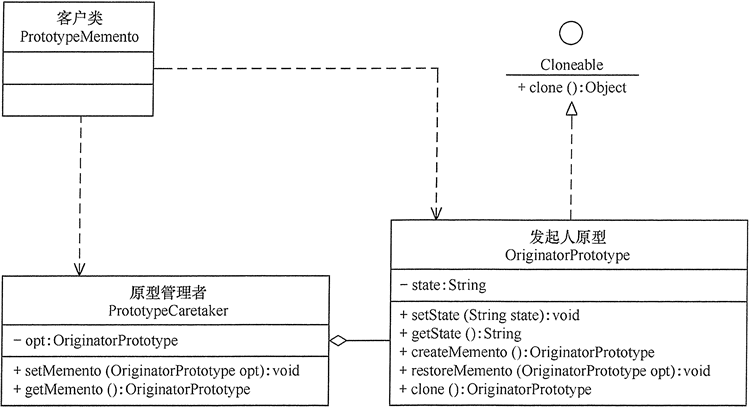
\includegraphics[width=0.8\textwidth]{image/18-4}
	\caption{带原型的备忘录模式的结构图}
\end{figure}
\begin{lstlisting}
//发起人原型
class OriginatorPrototype implements Cloneable {
	private String state;
	public void setState(String state) {
		this.state = state;
	}
	public String getState() {
		return state;
	}
	public OriginatorPrototype createMemento() {
		return this.clone();
	}
	public void restoreMemento(OriginatorPrototype opt) {
		this.setState(opt.getState());
	}
	public OriginatorPrototype clone() {
		try {
			return (OriginatorPrototype) super.clone();
		} catch (CloneNotSupportedException e) {
			e.printStackTrace();
		}
		return null;
	}
}
\end{lstlisting}
\begin{lstlisting}
//原型管理者
class PrototypeCaretaker {
	private OriginatorPrototype opt;
	public void setMemento(OriginatorPrototype opt) {
		this.opt = opt;
	}
	public OriginatorPrototype getMemento() {
		return opt;
	}
}
\end{lstlisting}
\begin{lstlisting}
public class PrototypeMemento {
	public static void main(String[] args) {
		OriginatorPrototype or = new OriginatorPrototype();
		PrototypeCaretaker cr = new PrototypeCaretaker();
		or.setState("S0");
		System.out.println("初始状态:" + or.getState());
		cr.setMemento(or.createMemento()); //保存状态
		or.setState("S1");
		System.out.println("新的状态:" + or.getState());
		or.restoreMemento(cr.getMemento()); //恢复状态
		System.out.println("恢复状态:" + or.getState());
	}
}
\end{lstlisting}
\section{扩展思路}
\begin{enumerate}
	\item Java的可见性
	\begin{itemize}
		\item public: 所有类都可以访问
		\item protected: 同一包中的类或是该类的子类可以访问
		\item default: 同一包中的类可以访问
		\item private: 只有该类可以访问
	\end{itemize}
	\item 需要Memento的个数:可以保存多个。
	\item Memento有效期:可以设置有效期,但要考虑程序升级兼容。
	\item Caretaker和Originator:Caretaker决定何时拍摄快照、何时撤销;
	当需求变更时,可以不用修改Originator。
\end{enumerate}
\section{相关设计模式}
\begin{enumerate}
	\item Command模式:结合Memento实现命令撤销;
	\item Protype模式:在Memento中,为了能够实现快照和撤销,保存对象当前状态,保存的信息只是在恢复状态时所需要的那部分信息;
	在Protype中,会生成一个与当前实例相同的实例。
	\item State模式:在Memento中,是用“实例”表示状态;在State中用类表示状态。
\end{enumerate}